\documentclass[10pt,a4paper,oneside]{article}

\usepackage[a4paper, margin=1in]{geometry}
\usepackage[utf8]{inputenc}
\usepackage[T1]{fontenc}
\usepackage[english]{babel}
\usepackage{graphicx}
\usepackage{hyperref}
\usepackage{xcolor}
\usepackage{amsmath}
\usepackage{cleveref}
\usepackage{subcaption}
\usepackage{booktabs}
\usepackage{multirow}
\usepackage{placeins}
\usepackage{float} 
\usepackage{comment}
\usepackage{lipsum}
\usepackage{minted}

\bibliographystyle{IEEEtran}

% Document metadata
\title{Classical ML for language identification}
\author{Yannik Queisler, Olivia Martin}
\date{\today}

\begin{document}

\maketitle
\begin{abstract}
\noindent Language identification (LID) is a fundamental problem in natural language processing (NLP) that involves determining the language of a given text. In this work, we frame LID as a multiclass classification task and evaluate classical machine learning approaches, including naïve Bayes, support vector machines (SVM), and logistic regression. Using a preprocessed subset of the WiLI-2018 dataset, we conduct hyperparameter selection over $n$-gram representation (character vs. word), vocabulary size, and additional noise removal. We report vocabulary coverage, accuracy, and macro F1-score as evaluation metrics. Our results indicate that SVM with character unigrams, a vocabulary size of 500, and no additional preprocessing achieves the highest accuracy and F1-score of 0.97. All models demonstrate strong overall performance, suggesting that traditional ML methods remain effective for LID. However, closely related languages, such as those in the Romance family, pose challenges, highlighting potential areas for improvement through deep learning techniques. The full codebase and experimental notebooks are publicly available on GitHub.\footnote{\url{https://github.com/devWhyqueue/lang-lens}}
\end{abstract}

% Table of contents
\thispagestyle{empty}
\setcounter{tocdepth}{2}
\tableofcontents
\newpage
\setcounter{page}{1}

% Sections
\section{Introduction}\label{sec:intro}

LID is the problem of determining the natural language that a given text, or part of it, is written in. It is a fundamental task in NLP that enables technologies such as multilingual search, speech recognition, and content filtering. As global content becomes increasingly diverse, the need for accurate and efficient LID systems grows. \cite{Jauhiainen2019}

Even though language identification has been extensively studied, it continues to pose challenges. For example, short texts (e.g., social media posts) may contain too little information for reliable classification. Code-switching, where multiple languages appear within a single sentence, can confuse models built for strictly monolingual text. Closely related languages or dialects (e.g., Serbian vs.\ Croatian) can also share significant lexical and syntactic similarities, making them difficult to distinguish. \cite{Vatanen2010}

In this project, however, our objective is not to develop a state-of-the-art LID system. Instead, we focus on evaluating and analyzing classical machine learning methods under realistic conditions, including noisy, multi-domain, and mixed-language data.

Specifically, we employ straightforward, interpretable techniques, such as character- or word-based $n$-gram models, and examine how different hyperparameters  (preprocessing, vocabulary size) affect their performance. Beyond raw accuracy and F1-score, we aim to understand how these configurations influence vocabulary coverage, error patterns, and overall model behavior -- thus providing deeper insights into the strengths and limitations of classical LID methods.
\section{Problem}\label{sec:problem}

We formulate LID as a multiclass classification task: given an input text, assign it exactly one language label.

\subsection{Definition}\label{subsec:definition}
Let $L = \{l_1, l_2, \dots, l_K\}$ be a set of $K$ possible languages, and let $D$ be the input space consisting of text samples (e.g., character strings, sequences of words, or tokenized representations). Formally, each text sample $d \in D$ can be viewed as a sequence of tokens $d = (w_1, w_2, \dots, w_n)$. 

A labeled training dataset is typically available:
\[
    \{(d_i, l_i)\}_{i=1}^N,
\]
where $d_i$ denotes a text sample and $l_i \in L$ is the associated ground-truth label. The goal is to learn a classifier
\[
    f_\theta: D \to L,
\]
so that for each $d$, we predict the most likely label $\hat{l} = f_\theta(d)$. Model parameters $\theta$ are learned by minimizing a loss function $\mathcal{L}$ (e.g., cross-entropy) over the training data:
\[
    \theta^* = \arg\min_\theta \; \frac{1}{N} \sum_{i=1}^N \mathcal{L}\bigl(f_\theta(d_i), l_i\bigr).
\]
In practice, many classifiers output a probability distribution over labels, allowing a decision rule such as
\[
    f_\theta(d) = \arg\max_{l \in L} \hat{p}(l \mid d).
\]

\subsection{Approaches}\label{subsec:approaches}
Various approaches exist for LID:
\begin{enumerate}
    \item \textbf{Rule-based:} These methods rely on handcrafted linguistic rules and dictionaries. They are effective for clearly distinguishable languages but often fail for ambiguous or code-switched text.
    \item \textbf{Statistical:} Use statistical models to learn language-specific patterns from data. These models can be based on character $n$-grams, word frequencies, or other features. One of the most popular early works on LID by Cavnar and Trenkle employs a character $n$-gram frequency method to classify languages. \cite{CavnarTrenkle1994}
    \item \textbf{Traditional ML:} Classifiers such as naïve Bayes, SVMs, or logistic regression employ engineered features, e.g., n-grams or TF-IDF, to predict language labels. Current tools like \texttt{langdetect} or \texttt{langid} are based on these methods. \cite{Nakatani2010, LuiBaldwin2012}
    \item \textbf{Hybrid methods:} Combine rule-based and statistical approaches to improve performance. For example, \textit{lingua} combines a statistical $n$-gram model with a rule-based engine. \cite{Lingua2025}
    \item \textbf{Neural networks:} Neural architectures (e.g., feedforward, recurrent, or transformer-based) can learn complex multilingual representations from large-scale corpora. Examples include Facebook's \texttt{fastText} and Google's \texttt{CLD3}. The former uses word embeddings and the latter character $n$-grams which they combine with a neural network. \cite{JoulinEtAl2016, GoogleCLD3}
\end{enumerate}
As a classification problem, LID benefits from standard algorithmic and modeling techniques while also requiring careful handling of language-specific nuances, varying input lengths, and potential multi-label scenarios (e.g., code-switching). 

\section{Datasets}\label{sec:datasets}
Several corpora for LI have been published in the past years. The following list provides an overview of some of the most popular datasets.

\begin{itemize}
    \item \textbf{WiLI-2018:} The Wikipedia language identification dataset is a benchmark dataset designed for written language identification tasks. Introduced by Martin Thoma in 2018, it consists of 1,000 short texts for each of 235 languages, sourced from Wikipedia. The dataset includes a diverse range of languages, covering different writing systems and linguistic families. \cite{Thoma2018}
    \item \textbf{LTI LangID:} Large-scale dataset for language identification, covering over 1,266 languages with text data from diverse sources. It has been instrumental in training models for identifying both high- and low-resource languages. The dataset is particularly valuable for handling noisy, real-world text, making it a key resource for multilingual NLP research. \cite{Caswell2020}
    \item \textbf{Tatoeba:} Free collection of example sentences with translations designed to assist language learners. It is available in over 400 languages. The name "Tatoeba" is derived from Japanese, meaning "for example." The project is maintained by a community of volunteers through open collaboration, and its contributors are known as Tatoebans. \cite{Tatoeba2025}
    \item \textbf{OpenLID:} Introduced by Burchell et al. in 2023, is a curated resource designed to enhance LID across 201 languages. This dataset comprises monolingual text from diverse sources, including news articles, Wikipedia entries, religious texts, and more. To ensure data reliability, the authors conducted a manual audit of samples from each language and source. Both the dataset and the trained model are publicly available, providing valuable resources for the research community. \cite{Burchell2023}
    \item \textbf{LCC:} The Leipzig Corpora Collection is a multilingual corpus repository that includes a wide range of text data in over 200 languages. The collection is maintained by the Natural Language Processing Group at Leipzig University and is freely available for research purposes. The LCC is a valuable resource for training and evaluating language identification models. \cite{Goldhahn2012}
\end{itemize}

\subsection{Khan's WiLI-2018 subset}\label{subsec:wili2018}
The dataset used in this project is a subset of the WiLI-2018 dataset, focusing on a smaller number of languages. This subset includes 22 languages with 1,000 samples each, resulting in a total of 22,000 samples. The text length distribution is shown in \cref{fig:text_length_distribution}. The majority of texts fall between 100 and 500 characters, averaging around 350 characters.

\begin{figure}
    \centering
    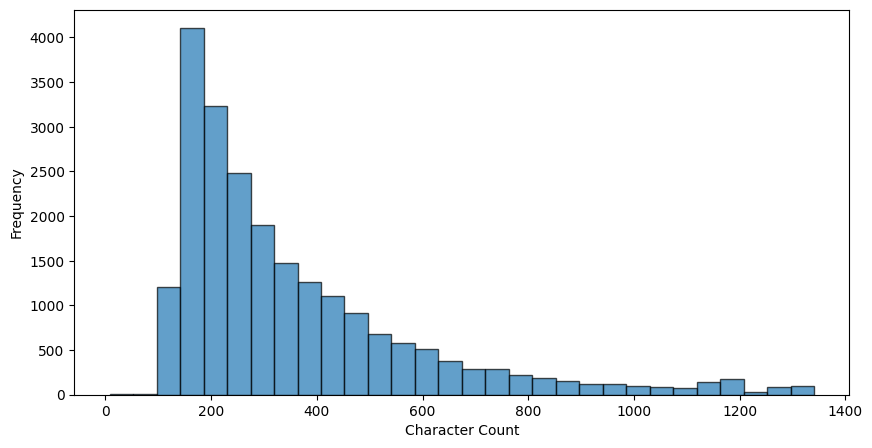
\includegraphics[width=0.8\textwidth]{figures/text_lengths.png}
    \caption{Text length distribution of the WiLI-2018 subset}
    \label{fig:text_length_distribution}
\end{figure}

A closer examination of the texts revealed 141 duplicate entries and one empty text. The duplicates are similarly present in the original dataset and were therefore retained, but the empty text appears to be a newly introduced error in the subset. The empty text was removed from the dataset. It likely originated from preprocessing, where the text was lowercased, and some noise removal was applied. However, the specifics are not disclosed by Khan, the author of the dataset on Kaggle. \cite{Khan2018}

While only a small fraction of the subset exactly matches the texts of the original (2.6\%), the majority (83.4\%) has a high similarity score (> 0.9) with the WiLI-2018 dataset. Similarity was measured using cosine similarity of TF-IDF vectors. 

\section{Hyperparameter selection}
The performance of LID models is highly dependent on the careful selection of hyperparameters. In this project, we fix unigrams as the feature representation to maintain consistency across experiments. The key hyperparameters considered include the choice of model, where we evaluate classical machine learning approaches such as naïve Bayes, SVM, and logistic regression. Additionally, we explore different $n$-gram types, including word-level and character-level representations. Other tunable parameters include the vocabulary size, which influences the feature space, and the application of preprocessing techniques, where we compare the effect of enabling or disabling text preprocessing steps.

\subsection{Models}
Several classical machine learning models are widely used for LID due to their effectiveness in handling text classification tasks. One of the most fundamental approaches is naïve Bayes, a probabilistic classifier based on Bayes' theorem with the assumption of feature independence. Despite this strong assumption, it performs well for text classification tasks due to the nature of word distributions in language data. SVM is another popular choice, which aims to find an optimal hyperplane that separates data points in a high-dimensional space, making it effective for text-based tasks when coupled with appropriate feature representations. Lastly, logistic regression is a linear model that predicts class probabilities using the sigmoid function, making it a simple yet effective approach for language classification. We use the implementations provided by the scikit-learn library for these models, which offer efficient and scalable solutions for text classification tasks. \cite{Hand2001, Cortes1995,cox1958regression}

\subsection{n-grams}
$n$-grams are widely used as feature representations in LID due to their ability to capture sequential patterns in text data. An $n$-gram is a contiguous sequence of $n$ elements from a given text, where these elements can be either words or characters. Word-level $n$-grams consider sequences of words, capturing syntactic and contextual information within a language. This approach is useful for languages with distinct word structures but may suffer from sparsity issues when dealing with large vocabularies. In contrast, character-level $n$-grams focus on sequences of individual characters, making them robust for handling morphologically rich languages, transliterations, and short texts. Character-level models are particularly effective in distinguishing languages with similar word distributions but differing orthographic or phonetic structures. While word $n$-grams offer greater interpretability and are beneficial for high-resource languages, character $n$-grams provide a more flexible and language-agnostic approach, making them a strong choice for multilingual and low-resource language identification tasks. \cite{CavnarTrenkle1994}

\subsection{Vocabulary size}
Vocabulary size impacts both the efficiency and effectiveness of text representation. The vocabulary consists of the unique tokens—either words or subword units—used to construct features for classification. A larger vocabulary captures more linguistic nuances and rare words, improving performance on diverse texts but also increasing computational cost and sparsity issues. Conversely, a smaller vocabulary reduces memory and computational requirements but may lead to a loss of discriminative power, especially in morphologically rich languages. The trade-off between vocabulary size and model performance has been extensively studied in the context of $n$-gram language models and neural word embeddings, where subword-level approaches such as character $n$-grams and byte pair encoding (BPE) help mitigate vocabulary limitations while preserving language-specific information. Careful selection of the vocabulary size is therefore essential to balance efficiency and accuracy in LID tasks.

\subsection{Preprocessing}
In general, multiple different preprocessing steps are viable for the LID task. Jauhiainen et al. mention the following preprocessing steps in their survey: \cite{Jauhiainen2019}

\begin{itemize}
    \item \textbf{Case folding}: Convert all characters to lowercase.
    \item \textbf{Range compression}: Groups a range of characters into a single logical set to reduce sparsity, which is especially useful for languages with large character sets like Chinese.
    \item \textbf{Noise removal}: Remove digits, punctuation, special characters, and language-independent characters (like URLs, emails, etc.). This is mostly done using heuristics.
\end{itemize}
Other common NLP preprocessing steps, however, might not be suited for the task. They mostly include normalization techniques:

\begin{itemize}
    \item \textbf{Removing stop words and diacritics}: As Truică et al. point out, stop words and diacritics are language-specific and useful for the LID task. \cite{Truic2018}
    \item \textbf{Lemmatization}: Relies on understanding a word's base form, which depends on grammar, morphology, and irregular forms.
    \item \textbf{Stemming}: Applies heuristic rules to chop off word endings, but these rules are language-dependent.
\end{itemize}
Language-agnostic approaches to these normalization techniques often rely on rule-based heuristics and are often impractical for numerous languages. Apart from these methods, one might use statistical, embedding-based or neural methods to learn word structures across languages. However, this would leave the realm of preprocessing for classical ML methods and enter the domain of deep learning.

As previously mentioned in \cref{subsec:wili2018}, Khan's WiLi-2018 dataset was already preprocessed. The text is already lowercased and some noise removal has been applied. As the dataset's name suggests, it is already optimized for the LID task. Therefore, we expect no significant performance improvements from further preprocessing. Nevertheless, we implement a preprocessing function introducing some further noise removal listed in \cref{lst:preprocessing} to validate that assumption.


\section{Results}
This section presents the evaluation of classical ML models' performances on Khan's WiLi-2018 subset. The evaluation is conducted using multiple standard metrics to assess its effectiveness in classifying languages. Note that this dataset poses a multiclass classification task. The results highlight the method's strengths and provide insights into areas requiring further improvement.

We include the metrics accuracy and macro F1-score. These metrics are widely used in the literature, allowing us to ensure that our results are comparable with existing studies. \cite{Jauhiainen2019}

\subsection{Evaluation metrics}
The metrics are defined as follows.

Accuracy measures the proportion of all classification instances that are classified correctly:

\begin{equation}
    \text{Accuracy} = \frac{\sum_{i} TP_i}{\sum_{i} (TP_i + FP_i + FN_i)},
\end{equation}
where $TP_i$, $FP_i$, and $FN_i$ are the true positive, false positive, and false negative instances for class $i$, respectively. 

Precision indicates the proportion of correctly classified instances among all instances classified as class $i$:

\begin{equation}
    P_i = \frac{TP_i}{TP_i + FP_i}
\end{equation}
Recall measures the amount of correctly positive classified instances proportionate to the true amount of positive classifications:

\begin{equation}
    R_i = \frac{TP_i}{TP_i + FN_i}
\end{equation}
The F1-score represents the harmonic mean of precision and recall:

\begin{equation}
    F1_i = \frac{2 \cdot P_i \cdot R_i}{P_i + R_i}
\end{equation}
The macro-averaged F1 treats all classes equally, offering insights into how well the model performs across all language classes, regardless of class imbalance.

\begin{equation} 
    \text{Macro F1} = \frac{1}{N} \sum_{i=1}^{N} F1_i
\end{equation}
In addition to the standard classification metrics, we also include the vocabulary coverage. This metric measures the proportion of tokens in a dataset that are covered by the vocabulary. A coverage of 100\% means that all tokens are included in the vocabulary. We will use the coverage as a measure of how well the vocabulary represents the data. Formally, the token-level coverage can be defined as follows:

\begin{equation}
    \text{Coverage} = \frac{\sum_{i=1}^{N} \mathbf{1} (t_i \in V)}{N},
\end{equation}
where $N$ is the number of tokens in the data, $t_i$ is the $i$-th token, and $V$ is the vocabulary.
 
\subsection{Findings}
\Cref{tab:performance} shows the performances different hyperparameter configurations for classical ML methods. They reveal important insights into the performance of the classifiers and the challenges inherent in the task. As we are performing hyperparameter selection, we evaluate on a separate validation set (10\%). Chosen model's final performance is reported on the test set (10\%). 
We summarize our main findings in this section.

\begin{table}[htbp]
    \centering
    \caption{Model performance on validation set across different configurations}
    \label{tab:performance}
    \begin{tabular}{llccrrrr}
        \toprule
        Model & N-gram & Vocab Size & Preproc. & Coverage & Accuracy & Macro F1 \\
        \midrule
        \multirow{8}{*}{Naive Bayes} 
        & \multirow{4}{*}{char} & 100 & No/Yes & 82\% / 85\% & 86\% / 86\% & 84\% / 84\%  \\
        & & 500 & No/Yes & 96\% / 96\% & 96\% / 97\% & 97\% / 97\%\\ 
        & & 1,000 & No/Yes & 98\% / 98\% & 96\% / 96\% & 96\% / 96\% \\
        & & 6,838 (max) & No/Yes & 100\% / 100\% & 94\% / 93\% & 94\% / 93\% \\
        \cmidrule{2-7}
        & \multirow{4}{*}{word} & 250 & No/Yes & 19\% / 21\% & 82\% / 77\% & 82\% / 77\% \\
        & & 1,000 & No/Yes & 27\% / 30\% & 90\% / 86\% & 89\% / 84\% \\
        & & 8,000 & No/Yes & 43\% / 48\% & 92\% / 87\% & 92\% / 86\%\\
        & & 64,000 & No/Yes & 61\% / 68\% & 94\% / 87\% & 94\% / 87\% \\
        \midrule
        \multirow{8}{*}{SVM}
        & \multirow{4}{*}{char} & 100 & No/Yes & 82\% / 85\% & 91\% / 91\% & 91\% / 90\% \\
        & & \textbf{500} & \textbf{No/Yes} & \textbf{96\% / 96\%} & \textbf{97\% / 97\%} & \textbf{97\% / 97\%} \\ 
        & & 1,000 & No/Yes & 98\% / 98\% & 97\% / 96\% & 97\% / 96\% \\
        & & 6,838 (max) & No/Yes & 100\% / 100\% & 97\% / 96\% & 97\% / 96\% \\
        \cmidrule{2-7}
        & \multirow{4}{*}{word} & 250 & No/Yes & 19\% / 21\% & 87\% / 82\% & 87\% / 82\% \\
        & & 1,000 & No/Yes & 27\% / 30\% & 94\% / 94\% & 94\% / 94\% \\
        & & 8,000 & No/Yes & 43\% / 48\% & 95\% / 90\% & 95\% / 89\% \\
        & & \textbf{64,000} & \textbf{No}/Yes & \textbf{61\%} / 68\% & \textbf{96\%} / 93\% & \textbf{96\%} / 92\% \\
        \midrule
        \multirow{8}{*}{Log. Reg.}
        & \multirow{4}{*}{char} & 100 & No/Yes & 82\% / 85\% & 90\% / 90\% & 89\% / 89\% \\
        & & 500 & No/Yes & 96\% / 96\% & 96\% / 95\% & 96\% / 95\% \\ 
        & & 1,000 & No/Yes & 98\% / 98\% & 96\% / 95\% & 96\% / 95\% \\
        & & 6,838 (max) & No/Yes & 100\% / 100\% & 96\% / 95\% & 96\% / 95\% \\
        \cmidrule{2-7}
        & \multirow{4}{*}{word} & 250 & No/Yes & 19\% / 21\% & 86\% / 82\% & 86\% / 82\%  \\
        & & 1,000 & No/Yes & 27\% / 30\% & 93\% / 89\% & 93\% / 89\% \\
        & & 8,000 & No/Yes & 43\% / 49\% & 94\% / 91\% & 94\% / 90\% \\
        & & 64,000 & No/Yes & 61\% / 68\% & 95\% / 91\% & 96\% / 91\%\\
        \bottomrule
        \end{tabular}
\end{table}

\paragraph{SVM performs best.}
All classical ML models perform well, with the best configurations of each model achieving accuracy/F1-scores above 0.95. Among them, SVM achieves the highest validation accuracy/F1 (0.97). When trained on both the training and validation sets, SVM yields a test accuracy/F1 of 0.96.\footnote{For comparability, we also trained this SVM configuration with an 80/20 train/test split. This yielded a test performance of accuracy/F1 of 0.97.} A possible explanation for the strong performance of even simple models is that the dataset is balanced, the texts have reasonable length, and the language subset is relatively small (22 languages). This finding aligns with comparable work like in the study of Bhansali et al.. \cite{Bhansali2022}

\paragraph{Character unigrams outperform word unigrams.}
Character unigrams outperform word unigrams, achieving the best validation accuracy/F1 of 0.97 compared to 0.96 for word unigrams. While this might not seem a notable difference at first, a comparison of the vocabulary sizes (500 vs. 64,000) shows the discriminative power difference of the two $n$-gram types. This difference is also evident in our PCA analysis (see \cref{fig:pca_svm_word_unigram} vs. \cref{fig:pca_svm_char_unigram}), where the explained variance of the first two principal components is much higher for character unigrams (46.6\%) than for word unigrams (6.7\%). As a result, the plot of character-based features appears more compact and exhibits better-separated clusters, while word-level features distribute their variance across thousands of dimensions, leading to less obvious clustering in two dimensions.

Character-level features often capture broad distinctions (e.g., different scripts) in fewer dimensions, making them particularly well-suited for language identification. In contrast, word-level features, though informative, are more prone to fragmentation—especially for languages with large or highly varied vocabularies—and thus require more dimensions to achieve similar separability.

\paragraph{PCA clusters show distinct language groups.}
A closer inspection of the PCA clusters (\cref{fig:pca_svm_char_unigram}) reveals three notable groupings:

\begin{enumerate}
  \item \textbf{European languages:} A cluster in the upper-right portion of the plot includes languages such as English, Spanish, Dutch, and Estonian. All of these use the Latin script and share many characters. In a two-dimensional PCA plot, they often overlap, indicating that additional dimensions are needed for finer separation.

  \item \textbf{Indo-Iranian and Semitic languages:} A cluster in the upper-left portion contains languages such as Arabic, Persian, Hindi, and Urdu, which share common script features (Arabic and its variants).

  \item \textbf{Asian languages:} A vertically stretched cluster in the middle consists of languages such as Chinese, Japanese, and Russian. These use distinct scripts with minimal character overlap (e.g., hanzi, kanji, Cyrillic), leading to a more dispersed distribution in the 2D plot.
\end{enumerate}

\paragraph{Coverage increases with vocabulary size.}
As vocabulary size increases, token coverage also increases. However, model performance does not consistently improve beyond a certain point. In fact, for character unigrams at the maximum vocabulary size, both accuracy and F1 decrease for naive Bayes. We hypothesize that introducing too many rare character sequences leads to overfitting, adding noise rather than improving discriminative power.

\paragraph{Further preprocessing has no further positive impact.}
We also experimented with more extensive noise removal. While this significantly increases coverage (especially for word unigrams), performance is either hardly affected for character unigrams or presents a notable decrease for word unigrams (96\% vs. 92\%). A plausible explanation is that the dataset is already well-prepared for language identification. In general, this task benefits from minimal rather than extensive preprocessing, particularly when working with relatively clean datasets. While preprocessing can be crucial in some cases, for this dataset, further cleaning does not yield performance gains. Note that hand-crafted rules taylored to this specific dataset might still improve performance but usually do not generalize well to other datasets and therefore do not improve the overall model.

\paragraph{Room for improvement with specific languages.}
Although the best model performs well overall, certain languages remain challenging. English, in particular, exhibits a high recall (0.95) but a comparatively low precision (0.81). From the confusion matrix (\cref{fig:matrix_svm_char_unigram}), we observe that instances of French, Estonian, Latin, and Spanish are misclassified as English. This is likely due to substantial character overlap between English and these languages, especially those in the Romance (French, Latin, Spanish) family. \cite{AbhishekPandey2023}

\section{Discussion}\label{sec:discussion}

In this section, we synthesize our key findings, delve into the broader implications of our results, and outline potential avenues for further improvement in LID.

\paragraph{Hyperparameters for LID.}
Our key hyperparameters were model choice, \(n\)-gram type (word vs.\ character), vocabulary size, and preprocessing. SVM performed best, likely due to its ability to handle high-dimensional sparse data. Character \(n\)-grams, especially unigrams, outperformed word-based features, capturing script and morphological patterns more effectively. Vocabulary size had an optimal range—too large, and rare tokens introduced noise. Additional preprocessing had minimal impact, as the dataset was already well-prepared, suggesting that extensive text cleaning is not always necessary for LID.

\paragraph{Is LID an easy task?}
Our findings might suggest that LID is relatively straightforward, given that simple, classical machine learning methods achieve high performance (over 0.95 F1 and accuracy in most configurations). However, this must be interpreted in the context of our dataset, which includes adequately long texts (reducing ambiguity), a balanced label distribution, and only 22 languages. As other studies have shown, language identification becomes markedly more challenging when dealing with much larger language sets or shorter text segments (e.g., social media posts). Thus, while our results demonstrate that classical ML approaches can perform well under controlled conditions, more complex scenarios demand more robust or specialized solutions. \cite{Jauhiainen2019}

\paragraph{Paths to improvement.}
Despite promising results with manual feature engineering, these methods have inherent limitations, especially as the language space expands or when dealing with highly variable and noisy data. Deep learning–based solutions, in particular transformer architectures such as XLM-RoBERTa, have shown the potential to handle more nuanced linguistic phenomena by leveraging large-scale multilingual pretraining. This allows them to capture deeper semantic and syntactic patterns without extensive hand-tuned feature extraction. \cite{AbhishekPandey2023}

% Appendix
\clearpage
\appendix
\section{Code}

\begin{listing}[h]
    \centering
    \begin{minipage}{0.9\textwidth}
        \begin{minted}[frame=single, fontsize=\footnotesize]{python}
def remove_noise(text: str) -> str:
    # Remove URLs
    text = re.sub(r'http\S+|www\.\S+', '', text)
    # Remove emails
    text = re.sub(r'\b[A-Za-z0-9._%+-]+@[A-Za-z0-9.-]+\.[A-Za-z]{2,}\b', '', text)
    # Remove digits
    text = re.sub(r'\d+', '', text)
    # Remove punctuation and special characters (excluding spaces)
    text = re.sub(r'[^\w\s]', '', text)
    # Remove extra spaces
    text = re.sub(r'\s+', ' ', text).strip()

    return text
        \end{minted}
    \end{minipage}
    \caption{Preprocessing function}
    \label{lst:preprocessing}
\end{listing}

\section{Visualizations}

\begin{figure}[h]
    \centering
    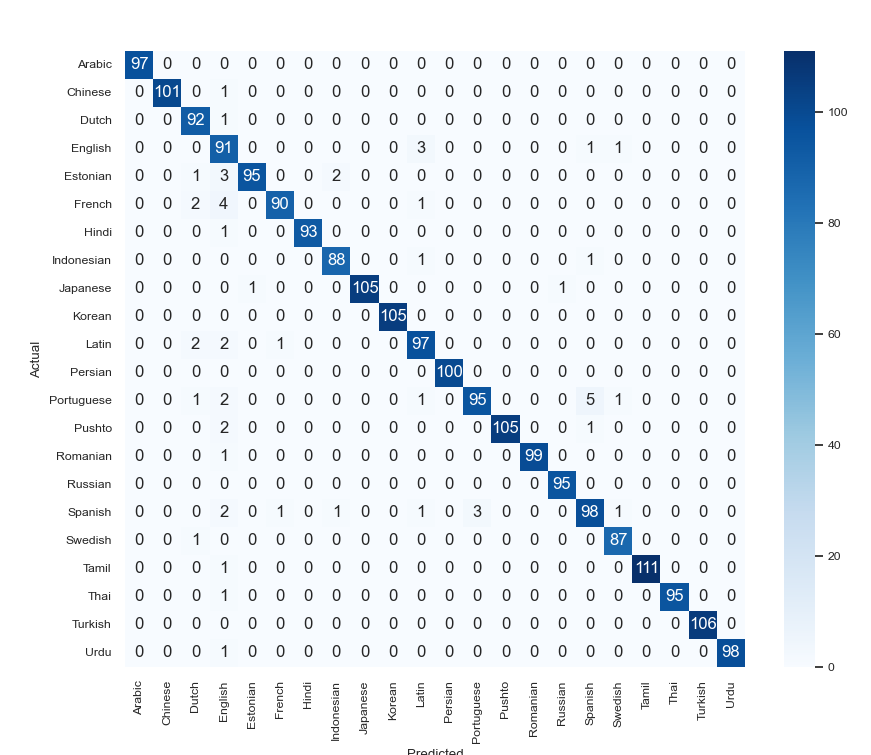
\includegraphics[width=0.8\textwidth]{figures/svm_char_unigram_val_set_matrix.png}
    \caption{Confusion matrix of the SVM model trained on the character unigram features}
    \label{fig:matrix_svm_char_unigram}
\end{figure}

\begin{figure}
    \centering
    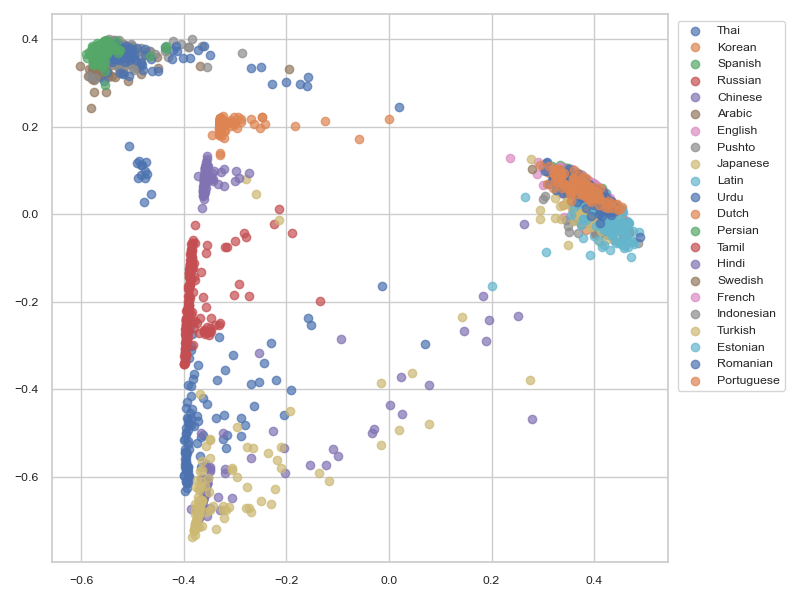
\includegraphics[width=0.9\textwidth]{figures/svm_char_unigram_val_set_pca.png}
    \caption{PCA visualization of the SVM model trained on the character unigram features}
    \label{fig:pca_svm_char_unigram}
\end{figure}

\begin{figure}
    \centering
    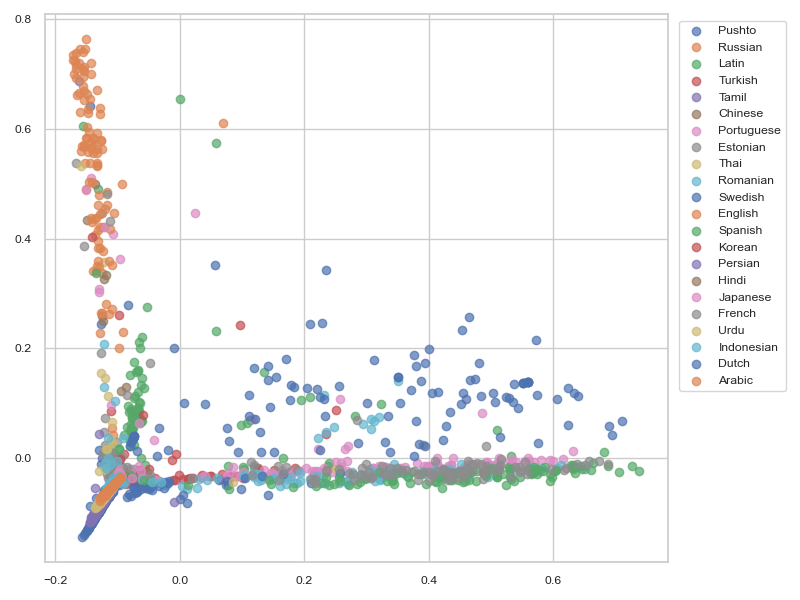
\includegraphics[width=0.9\textwidth]{figures/svm_word_unigram_val_set_pca.png}
    \caption{PCA visualization of the SVM model trained on the word unigram features}
    \label{fig:pca_svm_word_unigram}
\end{figure}




% References
\clearpage
\pagenumbering{gobble}
\bibliography{references}

\end{document}

